\begin{figure}[t!]
    \centering
    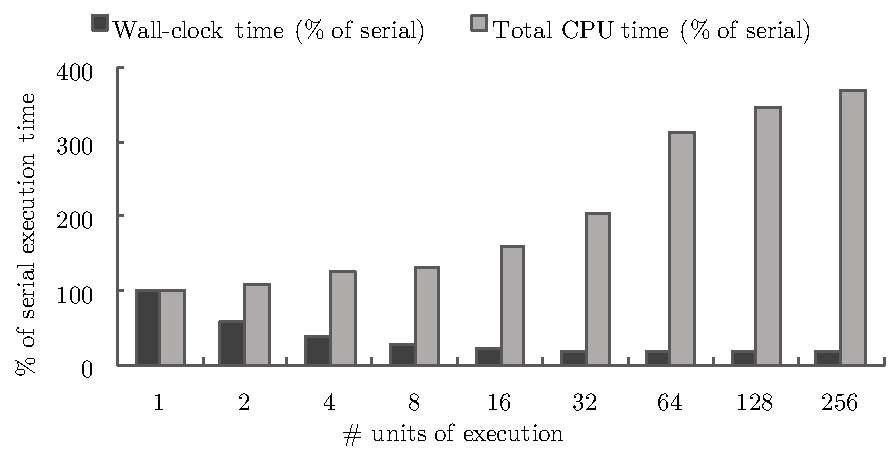
\includegraphics[width=8cm,height=4cm]{fig/speed-up.pdf}
    \caption{Wall-clock and total CPU execution times of the \texttt{bodytrack} application from the PARSEC benchmark suite~\cite{bienia2008parsec}. Increasing parallelism typically improves wall-clock execution time. However, total CPU time can increase, using more CPU resources to complete the same job. As an example, increasing from 16 to 32 threads increases total CPU time by approximately one-third, but we only see negligible improvement in wall-clock time.}
    \label{fig:speed-up}
\end{figure}